%% Copyright (C) M. Giordano, O. Iovino, M. Leccardi, 2010-2013
%%
%% Quest'opera è distribuita con licenza Creative Commons,
%%  + Attribuzione
%%  + Non commerciale
%%  + Condividi allo stesso modo
%% 3.0 Italia.
%%
%% Un riassunto in linguaggio accessibile a tutti della licenza è disponibile
%% alla pagina Internet http://creativecommons.org/licenses/by-nc-sa/3.0/it

\documentclass[b5paper,11pt,oneside]{guidatematica}
\ProvidesFile{guidaemacsauctex.tex}[2013/04/05 v.1.0.0 Breve guida all'uso di
Emacs per LaTeX]

\usepackage{guidaemacsauctex}

\begin{document}

\frontmatter

\title{Guida pratica all'uso\\ di\\ GNU Emacs e AUC\TeX}
\author{Mosè Giordano, Orlando Iovino, Matteo Leccardi}
\GetFileInfo{guidaemacsauctex.tex}
\date{\filename\ \fileversion\ del \filedate}
\maketitle

\chapter{Licenza d'uso}
\label{chap:licenza}

Quest'opera è soggetta alla Creative Commons Public License versione 3.0 o
posteriore: \emph{Attribuzione}, \emph{Non Commerciale}, \emph{Condividi allo
  stesso modo}. Un riassunto della licenza in linguaggio accessibile a tutti è
reperibile sul sito ufficiale
\url{http://creativecommons.org/licenses/by-nc-sa/3.0/deed.it}.

\bigskip\noindent\textsc{tu sei libero:}
\begin{itemize}
\item Di riprodurre, distribuire, comunicare al pubblico, esporre in pubblico,
      rappresentare, eseguire e recitare quest'opera.
\item Di modificare quest'opera.
\end{itemize}
\textsc{alle seguenti condizioni:}
\begin{itemize}
\item[\Large\ccAttribution] Devi attribuire la paternità dell'opera nei modi
      indicati dall'autore o da chi ti ha dato l'opera in licenza e in modo tale
      da non suggerire che essi avallino te o il modo in cui tu usi l'opera.
\item[\Large\ccNonCommercial] Non puoi usare quest'opera per fini commerciali.
\item[\Large\ccShareAlike] Se alteri o trasformi quest'opera, o se la usi per
      crearne un'altra, puoi distribuire l'opera risultante solo con una licenza
      identica o equivalente a questa.
\end{itemize}

\chapter{Presentazione}
\label{chap:presentazione}

\emacs\ è uno dei più vecchi e potenti editor di testi in circolazione e può
vantare fra i suoi utenti Donald Knuth, l'inventore di \TeX, e Leslie Lamport,
l'autore di \LaTeX.

\auctex, invece, è un pacchetto per \emacs\ scritto interamente in linguaggio
Emacs Lisp, che estende notevolmente le funzionalità di \emacs\ per produrre
documenti in \LaTeX\ e in altri formati legati al programma di tipocomposizione
\TeX.
% Fonti per Donald Knuth:
% https://www.informit.com/articles/article.aspx?p=1193856
% http://tex.loria.fr/litte/knuth-interview
% Fonte per Leslie Lamport:
% http://www.budiu.info/blog/2007/05/03/an-interview-with-leslie-lamport/
% Mihai Budui è un ricercatore della Microsoft
% (https://research.microsoft.com/en-us/people/mbudiu/), come Lamport, quindi
% l'intervista dovrebbe essere attendibile.

In questa guida tematica parleremo del programma \filestyle{GNU Emacs} (ovvero
del programma \emacs\ del progetto GNU, mentre non si accennerà alle sue diverse
varianti) e del pacchetto \auctex.  Si spiegherà come installarli e configurarli
sui tre principali sistemi operativi in circolazione (Windows, GNU/Linux e
Mac~OS), e come usarli per scrivere documenti \LaTeX.  Per finire si darà
qualche indicazione per personalizzare e rendere più efficiente \emacs.

Si tenga presente che, trattando di un programma così potente come \emacs, la
guida è ben lontana dall'essere esauriente.  Per ogni altro approfondimento non
riportato in queste righe rimandiamo il lettore ai manuali ufficiali, in
particolare a \cite{emacs:stallman} per \emacs\ e \cite{auctex:manual} per
\auctex.  Speriamo, con queste brevi note, di convincere il lettore che \emacs{}
non è poi così complicato come spesso viene considerato.

\section*{Colophon \& ringraziamenti}
\label{sec:colo:thanks}

Questa guida tematica è stata scritta a \emph{sei mani} grazie al sistema di
controllo di versione \progstyle{git}, che si scarica dal sito
\url{http://git-scm.com}. Chi vuole collaborare può ``clonare'' il progetto dal
deposito ufficiale presente sul sito \url{https://github.com/} alla pagina
\url{https://github.com/GuITeX/guidaemacsauctex}. Per compilare il codice
sorgente si consiglia di munirsi di una distribuzione \LaTeX\ aggiornata. È
inoltre necessario scaricare e installare nel proprio albero personale la classe
\classstyle{guidatematica} disponibile alla pagina
\url{https://github.com/GuITeX/guidatematica}.

Ringraziamo qui Tommaso Gordini per aver, da letterato qual egli è, reso il
testo più leggibile, oltre ad averci dato suggerimenti importanti per la
comprensione della guida.

È gradita ogni forma di collaborazione. Chiunque voglia segnalare errori,
refusi, commenti e suggerimenti può farlo agli indirizzi di posta elettronica
qui riportati.

\begin{flushright}
  \begin{minipage}{0.6\textwidth}\centering
    \textsc{Gli autori}                           \\[1.5ex]
    \textsc{Mosè Giordano}                        \\
    \texttt{giordano dot mose at libero dot it}   \\[0.5ex]
    \textsc{Orlando Iovino}                       \\
    \texttt{orlando dot iovino at yahoo dot it}   \\[0.5ex]
    \textsc{Matteo Leccardi}                      \\
    \texttt{matteo dot leccardi at gmail dot com} \\
  \end{minipage}
\end{flushright}

\newpage\tableofcontents*

\mainmatter

\chapter{Introduzione}
\label{chap:intro}

Lo sviluppo di \emacs{} è cominciato negli anni '70 del Novecento ai laboratori
di Intelligenza Artificiale del MIT, cioè molto prima che si diffondesse
l'informatica che conosciamo oggi.  Ciò comporta che \emacs{} utilizza una
terminologia spesso diversa da quella utilizzata dalla stragrande maggioranza
degli altri programmi che usiamo quotidianamente.  Perciò non bisogna
sorprendersi se l'operazione di \emph{tagliare} il testo (generalmente indicata
in inglese con \emph{cutting}) in \emacs{} viene chiamata \emph{killing} e
quella di \emph{incollare} il testo copiato (in inglese \emph{pasting}) viene
chiamata \emph{yanking}.

\emacs{} è famoso perché rende possibile eseguire \emph{qualsiasi} operazione
usando solo la tastiera, cioè senza l'ausilio del mouse.  A ogni comando può
essere associata una combinazione di tasti.  Sebbene questo fatto possa
inizialmente spaventare, è un vero punto di forza di \emacs{}, perché permette
di eseguire le operazioni in maniera rapida, invece di dover spostare il mouse
alla ricerca di appositi pulsanti.  In questa guida seguiremo la notazione
diffusa nel mondo di \emacs{} per indicare i tasti.  Quindi il tasto
\keys{\ctrl} verrà indicato con \verb!C!, l'\,\keys{Invio} con \verb!RET!, il
tasto \keys{\tab} con \verb|TAB|, mentre \verb!M! indica il tasto \keys{\Meta}
(sulle moderne tastiere quest'ultimo tasto è scomparso, ma si può ottenere lo
stesso risultato con \keys{\Alt} oppure premendo e rilasciando \keys{\esc}\,).
Nella notazione di queste scorciatoie, il trattino che separa due tasti in una
combinazione di tasti indica che i tasti vanno premuti contemporaneamente.
Così, quando si dirà che per eseguire un comando bisogna usare la combinazione
\verb!M-x!, si dovranno premere \emph{contemporaneamente} \keys{\Alt} e \keys{x}
oppure premere \keys{\esc}\,, rilasciarlo e premere \emph{successivamente}
\keys{x}\,.

Il manuale di \emacs~\citep{emacs:stallman} può essere consultato dall'interno
dello stesso programma con le combinazioni \verb!C-h r! (premere
contemporaneamente \keys{\ctrl} e \keys{h}\,, rilasciarli e premere
successivamente \keys{r}\,) oppure \verb!C-h i d m Emacs RET!  (premere
contemporaneamente \keys{\ctrl} e \keys{h}\,, rilasciarli e premere poi in
successione \keys{i}\,, \keys{d}\,, \keys{m}\,, scrivere successivamente
\verb!Emacs!, quindi premere \keys{Invio}\,).  Se si preferisce, si può
consultare il manuale anche tramite il menu
\menu{Help > Read the Emacs Manual}\,.

Una delle caratteristiche principali di \emacs{} è il fatto di essere un editor
di testi completamente personalizzabile ed espandibile, in modo da risultare
sempre adatto alle esigenze dell'utente.  Il linguaggio utilizzato per le
espansioni è l'Elisp, un dialetto del Lisp sviluppato appositamente per
\emacs{}.  Esistono migliaia di pacchetti scritti in Emacs Lisp che permettono
di estenderne ulteriormente le funzionalità.

La versione standard di \emacs{}, senza pacchetti aggiuntivi, fornisce già un
discreto supporto alla creazione di documenti \LaTeX, ma il pacchetto \auctex{}
mette a disposizione numerosi strumenti che rendono senza alcun dubbio \emacs{}
uno degli editor di testo più potenti in questo senso. In
questa guida vedremo alcune delle funzioni principali di \auctex.

Per finire, prima di addentrarci nell'installazione e nell'utilizzo di \emacs,
\auctex{} e di altri programmi accessori, è utile riportare qui qualche indicazione
sul file di inizializzazione di \emacs, scritto in Elisp e di fondamentale
importanza per modificare il comportamento delle funzioni del programma.  Questo
file, che sarà richiamato spesso in questo documento, presenta diversi nomi e
localizzazioni a seconda del sistema operativo usato.  Deve essere creato perché
inizialmente non esiste ed in particolare:
\begin{itemize}[leftmargin=*]
\item su Windows si chiama \filestyle{init.el} e va messo in
      \begin{itemize}[leftmargin=*]
      \item \verb|C:\Documents and Settings\|\meta{nome
              utente}\verb|\Dati Applicazioni\| (fino a XP);
      \item \verb|C:\Users\|\meta{nome utente}\verb|\AppData\.emacs.d\init.el|
            (da Vista in poi);
      \end{itemize}
\item su GNU/Linux e Mac~OS si chiama \filestyle{.emacs} o \filestyle{init.el} e
      va messo in \verb|~/.emacs|, \verb|~/.emacs.el| oppure in
      \verb|~/.emacs.d/init.el|.
\end{itemize}
Nelle prossime pagine ci riferiremo spesso al file di inizializzazione chiamandolo
semplicemente \verb|.emacs|, indipendentemente dalla posizione in cui si trova e
dall'effettivo nome utilizzato nel proprio sistema (\verb|.emacs|,
\verb|.emacs.el| oppure \verb|init.el| che sia).

Si faccia attenzione quando si copia e incolla il codice da questo documento:
potrebbe essere necessario riscrivere i caratteri \verb|"| e \verb|'| in \emacs.

%% --------------------------------------------------------------------------
%% Windows
%% --------------------------------------------------------------------------

\chapter{Installare \emacs{} e AUCTeX}
\label{chap:installazione}

\section{Windows}
\label{oi:sec:windows}

\subsection{Installare \emacs}
\label{oi:sec:installemacs}

Per sistemi operativi Microsoft Windows non esiste una vera e propria procedura
di installazione. \emacs{} si può utilizzare semplicemente procurandosi
l'archivio che ne contiene gli eseguibili.

All'indirizzo \url{http://ftp.gnu.org/pub/gnu/emacs/windows/} si scarichi
l'archivio compresso \filestyle{emacs-24.2-bin-i386.zip} e lo si decomprima in
una posizione di comodo; una buona soluzione, per esempio, è decomprimerlo
in \directory{C:/Programmi/Emacs/}, che assumeremo da questo
momento come cartella d'installazione.

Se si vuole creare un collegamento di \emacs{} nel menù Start, è sufficiente
eseguire il programma \progstyle{addpm.exe} contenuto nella cartella
\directory{C:/Programmi/Emacs/bin}.

A questo punto \emacs{} è pronto per scrivere documenti in \LaTeX: l'utente
infatti non deve specificare nessun percorso degli eseguibili della
distribuzione \LaTeX\ installata perché \emacs{} li trova da solo.

\subsection{Installare AUC\TeX}
\label{oi:sec:installauctex}

Si scarichi l'archivio compresso \filestyle{auctex-11.87-e24.2-msw.zip}
dall'indirizzo \url{http://www.gnu.org/software/auctex/download-for-windows} e
lo si decomprima in \directory{C:/Programmi/Emacs/}.  Si noti che alcuni file
sono gli stessi, perciò basta unire il contenuto dell'archivio di \auctex{} con
quello di \emacs.

Dopo aver installato \auctex, \emacs{} caricherà da solo i file necessari per
attivare la modalità \verb!latex-mode!, propria di \auctex, quando si apre o si
crea un file con estensione \filestyle{.tex}.

\subsection{Correttore ortografico}
\label{oi:sec:aspell}

Per usare il correttore ortografico in \emacs{} si deve installare il programma
\progstyle{GNU Aspell} disponibile all'indirizzo
\url{http://aspell.net/win32/}. L'ultima versione stabile è la 0.50-3 del
dicembre 2002.

Si devono installare, nell'ordine:
\begin{enumerate}
\item il programma \progstyle{Aspell-0-50-3-3-Setup.exe};
\item il dizionario precompilato per l'italiano \progstyle{Aspell-it-0.50-2-3.exe}.
\end{enumerate}

Infine rimane da eseguire qualche altra operazione:
\begin{enumerate}
\item Si deve copiare il
percorso della cartella dove sono contenuti gli eseguibili di \progstyle{Aspell}
nella variabile d'ambiente \textsf{PATH}.
\item Si deve aggiungere al proprio file
\filestyle{.init} le seguenti righe:
\begin{lstlisting}
(setq-default ispell-program-name "aspell")
(setq-default ispell-extra-args '("--reverse"))
(setq ispell-dictionary "italiano")
\end{lstlisting}
dove  la prima e la terza sono quelle strettamente necessarie, mentre la seconda
serve a risolvere gli eventuali problemi presentati dalle versioni precedenti
del programma.
\end{enumerate}

\subsection{Sincronizzare sorgente e anteprima}
\label{oi:sec:ricdirinv}

Prima di attivare la sincronizzazione tra il testo sorgente e l'anteprima del
documento, si spiega come risolvere il problema dei diritti di amministratore
--~qualora l'account utente ne sia fornito~-- per i sistemi operativi Vista e 7
(su XP non dovrebbero esserci problemi, mentre su Windows 8 non è stato
possibile provarlo). Infatti, in tale situazione si potrebbero avere problemi
con la cartella \directory{server} del tipo
\begin{lstlisting}[keywordstyle=\color{black}]
error: The directory '~/.emacs.d/server' is unsafe
\end{lstlisting}

Una possibile soluzione, riportata in~\cite{setupwindows}, è la seguente. Si
apra il prompt dei comandi e ci si porti nella cartella che contiene a propria
volta la cartella \directory{server}, scrivendo nella riga di comando
un'istruzione del tipo
\begin{lstlisting}[language=bash]
cd C:/Users/£\meta{nome utente}£/Roaming/.emacs.d
\end{lstlisting}
oppure
\begin{lstlisting}[language=bash]
cd %APPDATA%/.emacs.d
\end{lstlisting}
e infine
\begin{lstlisting}
takeown /f server
\end{lstlisting}
Il successo dell'operazione verrà segnalato con qualcosa come
\begin{lstlisting}
OPERAZIONE RIUSCITA: il file o la cartella ...
\end{lstlisting}

Si può ora configurare \emacs{} per la sincronizzazione con il
visualizzatore \progstyle{Sumatra~PDF} --~l'unico in grado di supportarla
nei sistemi Windows~-- scaricabile dal sito
\url{http://blog.kowalczyk.info/software/sumatrapdf/free-pdf-reader.html}.

Per la ricerca diretta basta scrivere nel file d'inizializzazione
\filestyle{.init}
\begin{lstlisting}
(setq TeX-source-correlate-method (quote synctex))
(setq TeX-source-correlate-mode t)
(setq TeX-source-correlate-start-server t)

(setq TeX-view-program-list
      '(("Sumatra PDF" ("\"C:/Program Files (x86)/\
SumatraPDF/SumatraPDF.exe\" -reuse-instance"
	  (mode-io-correlate " -forward-search %b %n") " %o"))))

(setq TeX-view-program-selection
      '(((output-dvi style-pstricks) "dvips and start")
	(output-dvi "Yap")
	(output-pdf "Sumatra PDF")
	(output-html "start")))
\end{lstlisting}

Per la ricerca inversa, invece, si apra \progstyle{Sumatra~PDF}, si raggiunga
il menù \menu{Impostazioni > Opzioni\dots} e si scriva
\begin{lstlisting}[flexiblecolumns]
C:/Programmi/Emacs/bin/emacsclientw.exe --no-wait +%l "%f"
\end{lstlisting}
in \textsf{Imposta la ricerca inversa via riga di comando}, come si vede dalla
figura~\ref{oi:fig:sumatra:setup}.
\begin{figure}[t]
  \centering
  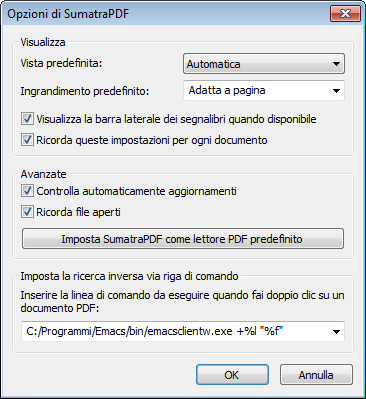
\includegraphics[width=0.50\textwidth]{sumatrapdf}
  \caption{Impostazioni per il visualizzatore \progstyle{Sumatra~PDF}.}
  \label{oi:fig:sumatra:setup}
\end{figure}

Con queste impostazioni il visualizzatore predefinito per \emacs\ -- ma non del
sistema operativo -- sarà \progstyle{Sumatra~PDF}.  Per la ricerca diretta vanno
premuti i tasti \verb!C-c C-v! e il visualizzatore si aprirà (o porterà) in
corrispondenza della riga del testo sorgente in cui si trova il cursore.  Per la
ricerca inversa, invece, basta un doppio clic nel visualizzatore.

%% --------------------------------------------------------------------------
%% GNU/Linux
%% --------------------------------------------------------------------------

\section{GNU/Linux}
\label{mg:sec:linux}

\subsection{Installare \emacs}
\label{mg:sec:installemacs}

\emacs{} fa parte del progetto GNU, quindi è presente nei depositi di tutti i
sistemi operativi della famiglia GNU/Linux.  Se non fosse già installato, il
metodo più semplice per ottenerlo è tramite il gestore di pacchetti della
propria distribuzione (naturalmente, si possono utilizzare anche i gestori di
pacchetti a interfaccia grafica).  Riportiamo qui i comandi da terminale utili
per installare il programma in alcune delle principali distribuzioni.

Su Debian e Ubuntu:
\begin{lstlisting}
$ sudo apt-get install emacs
\end{lstlisting}
Su Fedora:
\begin{lstlisting}
$ sudo yum install emacs
\end{lstlisting}
Su OpenSUSE:
\begin{lstlisting}
$ sudo zypper install emacs
\end{lstlisting}

Il metodo più difficile, per i non avvezzi al terminale, consiste nel compilare
\emacs{} a partire dal codice sorgente, ma non è intenzione di questa guida
spiegare come farlo.

Dopo aver installato \emacs, lo si potrà avviare facendo clic sul suo
\emph{launcher} oppure eseguendo da terminale il comando
\begin{lstlisting}
$ emacs
\end{lstlisting}
Se si desidera utilizzare \emacs{} con interfaccia testuale bisogna aggiungere
al comando appena visto l'opzione \texttt{-nw} oppure
\texttt{--no-window-system}:
\begin{lstlisting}
$ emacs -nw
\end{lstlisting}
Come argomento da linea di comando si può aggiungere il nome del file o dei file
che si vogliono modificare:
\begin{lstlisting}
$ emacs file1.tex file2.tex
\end{lstlisting}

\subsection{Installare AUC\TeX}
\label{mg:sec:installauctex}

Di solito anche il pacchetto \auctex{} è presente nei depositi dei sistemi
GNU/Linux.  Come già detto per \emacs{} si consiglia di installarlo con il
gestore di pacchetti della propria distribuzione.  Ecco i comandi da usare nelle
principali distribuzioni.

Su Debian e Ubuntu:
\begin{lstlisting}
$ sudo apt-get install auctex
\end{lstlisting}
Su Fedora:
\begin{lstlisting}
$ sudo yum install emacs-auctex
\end{lstlisting}
Su OpenSUSE:
\begin{lstlisting}
$ sudo zypper install emacs-auctex
\end{lstlisting}

Sulle prime due il gestore potrebbe raccomandare di installare la TeX~Live
presente nei depositi ufficiali del sistema operativo.  Per evitare che questo
avvenga, per esempio perché si utilizza una TeX~Live installata in altro modo,
installando \auctex{} da terminale è sufficiente aggiungere l'opzione
\verb!--no-install-recommends!:
\begin{lstlisting}
$ sudo apt-get install --no-install-recommends auctex
\end{lstlisting}

\subsection{Correttore ortografico}
\label{mg:sec:aspell}

Il correttore ortografico \progstyle{GNU Aspell} può essere installato
facilmente su GNU/Linux utilizzando, come al solito, il gestore di pacchetti
della propria distribuzione. Il dizionario italiano di \progstyle{GNU Aspell}
per GNU/Linux si chiama \progstyle{aspell-it}, quindi in Debian si installa da
terminale con il comando
\begin{lstlisting}
$ sudo apt-get install aspell-it
\end{lstlisting}
in Fedora con
\begin{lstlisting}
$ sudo yum install aspell-it
\end{lstlisting}
mentre in openSUSE si può dare
\begin{lstlisting}
$ sudo zypper install aspell-it
\end{lstlisting}


%% --------------------------------------------------------------------------
%% Mac OS
%% --------------------------------------------------------------------------

\section{Mac OS}
\label{ml:sec:linux}

\subsection{Installare \emacs}
\label{ml:sec:installemacs}

Sul mirror ufficiale \url{http://ftp.gnu.org/pub/gnu/emacs/} non è presente una
versione di \emacs{} già compilata per Mac OS X, perché queste versioni sono
rese disponibili da vari volontari come per esempio il gestore del sito
\url{http://emacsformacosx.com/}.  La procedura d'installazione è quella
consueta: dopo aver scaricato la versione più recente, si apra il file
\filestyle{.dmg} (se non è già stato aperto automaticamente al termine del
download) e si trascini l'icona di \emacs{} nella cartella
\directory{Applicazioni}.

In Mac OS le applicazioni avviate dall'interfaccia grafica non hanno
accesso ai valori delle variabili d'ambiente, per cui bisogna rendere
disponibile a \emacs{} la variabile \texttt{PATH} dando da terminale
il comando
\begin{lstlisting}[language=bash]
$ defaults write ~/.MacOSX/environment PATH "$PATH"
\end{lstlisting}
Si noti che le nuove impostazioni saranno effettive solo dopo aver eseguito un logout e un
successivo login. Il comando va ripetuto ogni volta che si installa un programma
che modifica il valore di \texttt{PATH}. (il caso che
riguarda più da vicino i lettori di questa guida è la distribuzione \TeX).

% TODO: controllare che i tasti inseriti con `\keys{}' siano corretti
Per gli utenti che usano la tastiera italiana è utile impostare il
tasto \keys{\cmdmac} come \keys{\Meta} e il tasto \keys{\Altmac} per
scrivere i caratteri speciali (in particolare parentesi quadre,
graffe e tilde) scrivendo queste righe nel file \filestyle{.emacs}:
\begin{lstlisting}
(setq ns-command-modifier 'meta)
(setq ns-alternate-modifier nil)
\end{lstlisting}

\subsection{Correttore ortografico}
\label{ml:sec:aspell}

Anche per Mac OS X è disponibile una versione di \progstyle{GNU Aspell}, chiamata
\progstyle{cocoAspell}, e disponibile all'indirizzo
\url{http://cocoaspell.leuski.net/}.

Dopo aver installato la versione 2.1 (a oggi l'ultima versione) si possono
scaricare i dizionari delle lingue che interessano direttamente
dal sito di \progstyle{GNU Aspell}, all'indirizzo
\url{ftp://ftp.gnu.org/gnu/aspell/dict/}. Quello italiano, per esempio, si chiama
\href{ftp://ftp.gnu.org/gnu/aspell/dict/it/aspell6-it-2.2_20050523-0.tar.bz2}%
{\filestyle{aspell6-it-2.2\_20050523-0.tar.bz2}}.

A questo punto bisogna estrarre il contento
degli archivi in una cartella temporanea, aprire una sessione di
terminale e portarsi nella cartella appena creata. I dizionari si
installano dando i comandi
\begin{lstlisting}
$ ./configure
$ make
$ sudo make install
\end{lstlisting}

Infine si deve configurare \emacs\ aggiungendo al file
\filestyle{.emacs} le righe
\begin{lstlisting}
(setq-default ispell-program-name "aspell")
(setq ispell-dictionary "italiano")
\end{lstlisting}

\subsection{Installare AUC\TeX}
\label{ml:sec:installauctex}

Come per \emacs, non è disponibile una versione di \auctex{} già compilata per
Mac~OS, ma purtroppo in questo caso non ne esistono neppure versioni non ufficiali. È quindi
necessario utilizzare il programma \progstyle{make}, che viene
installato insieme al  correttore ortografico
\progstyle{cocoAspell}, descritto nel paragrafo~\ref{ml:sec:aspell}.
Ecco le istruzioni.

Dalla pagina relativa a Mac OS X,
\url{http://www.gnu.org/software/auctex/download-for-macosx.html},
bisogna scaricare l'archivio compresso \filestyle{auctex-11.87.tar.gz}.  Se ne
estragga poi il contenuto in una cartella temporanea, si apra una sessione di
terminale e ci si porti nella cartella appena creata.  Bisogna poi configurare
\auctex{} con il comando
\begin{lstlisting}[flexiblecolumns, breaklines=false]
$ ./configure 
--prefix=/Applications/Emacs.app/Contents/Resources/ 
--with-emacs=/Applications/Emacs.app/Contents/MacOS/Emacs 
--with-lispdir=/Applications/Emacs.app/Contents/Resources/site-lisp/
--without-texmf-dir
\end{lstlisting}
sostituendo se necessario a \texttt{Applications}\footnote{Utilizzando il
  terminale non bisogna utilizzare i nomi localizzati delle cartelle ma quelli
  reali, quindi \texttt{Applications} è corretto anche se si utilizza la
  versione italiana di Mac OS.} la cartella in cui si trova \emacs. In questo
modo tutti i file saranno contenuti nel bundle \texttt{Emacs.app}. Il comando
precedente deve essere scritto nel terminale su una sola riga, sostituendo le
interruzioni di linea con spazi.

Infine si compili e si installi dando
\begin{lstlisting}
$ make && make install
\end{lstlisting}

Dopo l'installazione, bisogna impostare i visualizzatori per i vari file creati
con \LaTeX{} scrivendo nel file \filestyle{.emacs} queste righe
\begin{lstlisting}
(setq TeX-view-program-list
      '(("dvips and Skim" "%(o?)dvips %d -o &&\
  /Applications/Skim.app/Contents/SharedSupport/\
displayline %n %f %b")
	("Skim" "/Applications/Skim.app/Contents/\
SharedSupport/displayline %n %o %b")
        ("open" "open %o")))
(setq TeX-view-program-selection
      '(((output-dvi style-pstricks) "dvips and Skim")
        (output-dvi "Skim")
        (output-pdf "Skim")
        (output-html "open")))
\end{lstlisting}
Come visualizzatore si usa \progstyle{Skim},
\url{http://skim-app.sourceforge.net/}, perché supporta la sincronizzazione tra
sorgente e anteprima. La procedura di configurazione di \emacs{} e
\progstyle{Skim} è descritta nel paragrafo~\ref{ml:sec:ricdirinv}.

\subsection{Sincronizzare sorgente e anteprima}
\label{ml:sec:ricdirinv}

L'unico visualizzatore di file PDF per Mac~OS~X associato a \emacs{}
che supporti la sincronizzazione tra sorgente e anteprima  è
\href{http://skim-app.sourceforge.net/}{\progstyle{Skim}}
(si veda il paragrafo~\ref{ml:sec:installauctex}) che una volta installato
va configurato nel pannello \menu{Skim > Preferenze\dots > Sincronizza}
come segue e come mostra la figura~\ref{fig:skimpref}:
\begin{itemize}
\item si spunti la casellina \textsf{Controlla cambiamenti del file};
\item si scriva nel campo \textsf{Comando:}  \\
      \verb!/Applications/Emacs.app/Contents/MacOS/bin/emacsclient!
\item si scriva nel campo \textsf{Argomenti:} \verb!--no-wait +%line "%file"!
\end{itemize}
\begin{figure}[tb]
  \centering
  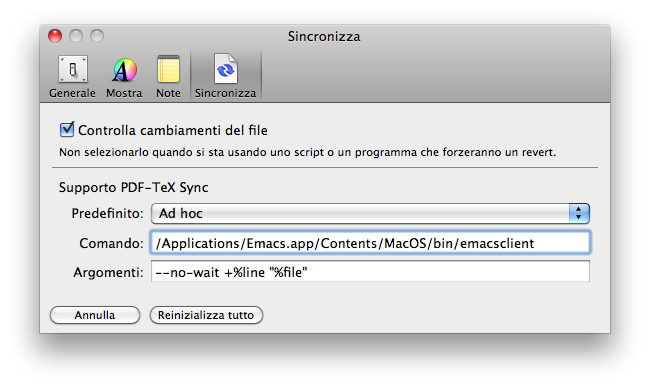
\includegraphics[width=\textwidth]{preferenze_skim}
  \caption{Preferenze di \progstyle{Skim} per sincronizzare sorgente e anteprima.}
  \label{fig:skimpref}
\end{figure}

La prima opzione fa in modo che quando un file aperto in \progstyle{Skim} viene
modificato da un altro processo, il programma chieda se il file modificato debba
essere ricaricato: scegliendo \textsf{Automatico}, i successivi aggiornamenti
verranno visualizzati senza chiedere ulteriori conferme.

\emacs{} si configura scrivendo nel file \filestyle{.emacs} le righe
\begin{lstlisting}
(setq TeX-source-correlate-method 'synctex)
(setq TeX-source-correlate-mode t)
(setq TeX-source-correlate-start-server t)
\end{lstlisting}

Si passa dal sorgente al PDF con la combinazione \verb!C-c C-v!; si ottiene il
contrario facendo clic sulla parola che interessa premendo contemporaneamente
\keys{\shift} e \keys{cmd}\,.

Se alcune versioni di \emacs{} precedenti alla 23.3 lasciassero in primo piano
la finestra del visualizzatore, si aggiungano queste righe al file
\filestyle{.emacs}
\begin{lstlisting}
(defun ns-raise-emacs ()
  (ns-do-applescript "tell application \"Emacs\" to activate"))
(add-hook 'server-switch-hook 'ns-raise-emacs)
\end{lstlisting}

\chapter{Primi passi in \emacs}
\label{chap:primi-passi-emacs}

Nei precedenti capitoli si è spiegato come installare e configurare i principali
componenti per usare \LaTeX\ con \emacs\ e \auctex. In questo capitolo vedremo
come si scrive in \emacs\ un semplice documento \filestyle{.tex} e come usare il
correttore ortografico.
% e come gestire gli errori.

\section{Ciao mondo}
\label{sec:primodocumento}

Ogni sistema operativo permette di aprire \emacs\ tramite un collegamento al
programma principale, dopo di che sullo schermo dovrebbe comparire la finestra
principale mostrata nella figura~\ref{fig:principale}.  Nel gergo di \emacs\ una
finestra è chiamata \emph{frame}.  Ciascun \emph{frame} può essere suddiviso in
una o più \emph{windows}, cioè lo spazio dove l'utente scrive, che è la zona di
principale interazione con il programma.  Un'altra componente fondamentale di un
\emph{frame} di \emacs, mostrata nella figura, è il \emph{minibuffer}.  Questo è
il posto dove \emacs\ dialoga con l'utente mostrando messaggi di notifica oppure
permettendo l'inserimento dell'input dei comandi eseguiti di volta in
volta~\citep{emacs:odebari}.  Il testo che si sta modificando in \emacs\ è
contenuto in un oggetto chiamato \emph{buffer}.  Quando si apre un file, il suo
testo viene memorizzato in un buffer.  In prima approssimazione possiamo dire
che il \emph{buffer} è il contenuto di un file, già esistente oppure che si sta
creando.

\begin{figure}[ht]
  \centering
  \begin{tikzpicture}\footnotesize\sffamily
    %
    % immagine
    %
    \pgfdeclareimage[width=0.70\textwidth]{splash}{figure/splash}
    \pgftext[at=\pgfpoint{0}{0},left,base] {\pgfuseimage{splash}};
    % \draw[help lines,step=0.1] (0,0) grid (0.70\textwidth,10);
    %
    % minibuffer
    %
    \draw[line] (8.2,0.15) -- (9,0.15) node[block,right=2] {minibuffer};
    %
    % window
    %
    \draw[line] (8.2,3.5) -- (9,3.5) node[block,right=2] {window};
    %
    % toolbar
    %
    \draw[line] (8.2,7) -- (10,7) -- (10,6.5) node[block,below=2] {toolbar};
    %
    % menubar
    %
    \draw[line] (8.2,7.4) -- (9,7.4) node[block,right=2] {menubar};
  \end{tikzpicture}
  \caption{Un \emph{frame} di \filestyle{GNU Emacs} che contiene la classica
    schermata iniziale.}
  \label{fig:principale}
\end{figure}

Terminata questa breve carrellata terminologica, possiamo passare alla pratica.
Per creare un nuovo documento ci sono due modi: raggiungendo il menù
\menu{File > Visit New File\dots} oppure premendo \verb|C-x C-f|, dopo di che
\emacs\ chiederà di aprire/trovare un file.  Scrivendo un nome che nella
cartella di lavoro non esiste questo file sarà creato. Dopo averlo nominato, per
esempio \filestyle{primo.tex}, si può cominciare a scrivere in \LaTeX.  Per gli
amanti delle scorciatoie da tastiera (autentico punto di forza di \emacs),
scrivendo \verb|C-c C-e| potremo inserire un nuovo ambiente in modo interattivo.
Il cursore si sposterà nel \emph{minibuffer} e lì si potrà scrivere il nome
dell'ambiente da inserire.  Questo è il messaggio visualizzato:
\begin{lstlisting}
Environment type: (default document)
\end{lstlisting}
In questo esempio, dato che non c'è ancora alcun documento attivo, l'ambiente
\ambstyle{document} sarà proposto come quello predefinito.  Dopo il primo
\verb|RET| apparirà nel minibuffer la scritta
\begin{lstlisting}
Document class: (default article)
\end{lstlisting}
che permette di scegliere la classe che, per impostazione predefinita, è
\classstyle{article}. Si dia ancora \verb|RET| e si vedrà
\begin{lstlisting}
Options:
\end{lstlisting}
che permette di scegliere le opzioni della classe.  Si faccia la scelta, si dia
un terzo \verb|RET| e si avrà infine il classico
\begin{lstlisting}[language={[LaTeX]TeX}]
\documentclass{article}

\begin{document}
£\meta{\textrm{cursore}}£
\end{document}
\end{lstlisting}
con il cursore correttamente posizionato nell'ambiente \ambstyle{document}.

Come è naturale che sia, le macro \LaTeX\ possono essere inserite manualmente,
ma \auctex\ facilità notevolmente il loro inserimento.  \auctex, infatti,
conosce la sintassi delle macro e degli ambienti di un centinaio dei pacchetti
\LaTeX\ più diffusi.  Per poter inserire una macro nel documento bisogna premere
\verb|C-c RET| e nel \emph{minibuffer} sarà possibile inserire il nome della
macro.  Si può utilizzare \verb|TAB| per l'autocompletamento.  Inoltre conosce
gli argomenti e le opzioni delle macro: infatti, dando \verb!C-c RET frac RET!
nel documento si otterrà \verb!\frac{}{}! e il cursore si posizionerà
all'interno del primo paio di parentesi graffe.  Analogamente, con
\verb!C-c RET sqrt RET! verrà richiesto l'ordine \verb!n! della radice da
inserire (premere direttamente \verb!RET! per non inserire nulla) e si otterrà
\verb!\sqrt[n]{}!.  Un altro esempio è la macro \verb|\verb|: \auctex\ chiederà
di scegliere il carattere da utilizzare come delimitatore e poi di inserire il
testo di argomento.

Per comporre il documento, si può
\begin{compactitemize}
\item premere sul pulsante presente nella \emph{toolbar};
\item scegliere \menu{Command > LaTeX}\,;
\item scrivere \verb|C-c C-c|. In quest'ultimo caso nel minibuffer si vedrà
\begin{lstlisting}
Command: (default LaTeX)
\end{lstlisting}
      e si dovrà premere \verb|RET| per lanciare effettivamente \LaTeX.
\end{compactitemize}
Durante la composizione del documento \emacs\ restituirà
\begin{lstlisting}
Type `C-c C-l' to display results of compilation.
\end{lstlisting}
e alla fine, se tutto è filato liscio senza errori, si avrà
\begin{lstlisting}
LaTeX: successfully formatted {1} page
\end{lstlisting}
Con questa procedura si scrive un nuovo documento \LaTeX.

Senza nessuna impostazione personale, il procedimento appena descritto
crea un file \filestyle{.dvi}. Se con gli stessi comandi
 si vuole invece un file \filestyle{.pdf}, si deve scrivere
\begin{lstlisting}
(add-hook 'LaTeX-mode-hook 'TeX-PDF-mode)
\end{lstlisting}
nel file \filestyle{.emacs}.

Per visualizzare il documento prodotto, sia esso un file \filestyle{.dvi} o un
\filestyle{.pdf}, si può
\begin{compactitemize}
\item premere sul pulsante presente nella \emph{toolbar};
\item raggiungere \menu{Command > View} e dare poi \verb|RET|;
\item scrivere \verb|C-c C-C RET| o \verb|C-c C-v|.
\end{compactitemize}
Se \emacs\ e \auctex\ sono configurati per lavorare con la sincronizzazione, in
tutti e tre i casi il visualizzatore dovrebbe aprirsi sulla riga corrispondente
del file sorgente.

\section{Correzione ortografica}
\label{sec:corr:orto:in:azione}

Dopo aver descritto le modalità di installazione dei correttori ortografici,
in questo paragrafo specifichiamo come usarli, indipendentemente dal sistema
operativo presente sulla propria macchina.

Per fare una revisione del documento che si sta scrivendo, bisogna dare
\verb!M-x ispell RET!: in questo modo il dizionario proporrà, in sequenza, la
correzione dei termini che trova errati.

Un secondo modo per scrivere correttamente è attivare la modalità
\emph{flyspell} (‘correzione al volo’). Se la si vuole solo sul documento
corrente, basta andare in
\menu{Tools > Spell Checking > Automatic spell checking (Flyspell)}; se invece
la si vuole sempre abilitata si deve aggiungere la riga
\begin{lstlisting}
(add-hook 'LaTeX-mode-hook 'flyspell-mode)
\end{lstlisting}
al proprio file \filestyle{.emacs}.

Quando il correttore rileva una parola potenzialmente non corretta, la colora
(in genere) in rosso. Alcuni termini, però, vengono segnalati come scorretti
anche quando non lo sono, ma solo perché non sono presenti nel dizionario: vi
possono essere aggiunti portando il puntatore del mouse sulla parola in
questione, premendo il tasto centrale e scegliendo \texttt{Save word}.

\chapter{Uso avanzato di \emacs}
\label{chap:uso:avanzato}

\section{Un documento più complesso}
\label{sec:documento:complesso}

Per scrivere documenti piuttosto corposi come libri, manuali, tesi e così via,
conviene suddividere il documento in un file principale, che chiameremo per
esempio \filestyle{master.tex}, e altri file nei quali scrivere il vero e
proprio contenuto del lavoro, per esempio \filestyle{capitolouno.tex} e
\filestyle{capitolodue.tex}.

\emacs, come altri editor di testi, permette di lanciare la composizione del
documento direttamente dal file su cui si sta lavorando anche se questo non è il
file principale, cioè il file \filestyle{master.tex} che dovrà contenere, per
definizione, qualcosa come
\begin{lstlisting}[language={[LaTeX]TeX}]
\documentclass{book}

\begin{document}

\input{capitolouno}
\input{capitolodue}

\end{document}

%%% Local Variables:
%%% mode: latex
%%% TeX-master: t
%%% End:
\end{lstlisting}

Si notano subito alcune righe commentate non presenti nel codice descritto nel
paragrafo~\ref{sec:primodocumento}: sono le \emph{variabili locali}.  Per capire
subito di che cosa si tratti, si pensi alle famose ‘righe magiche’ che si usano
per esempio con \TeX works~\citep{texworks:gregorio}.

Le variabili locali sono metacommenti ignorati da \LaTeX\ --~in quanto
commenti~-- ma non da \emacs\ e servono per impostare alcune preferenze del
documento in lavorazione.  Esse si possono indicare alla fine del file tra le
righe \verb|%%% Local Variables:| e \verb|%%% End:| oppure in un'unica riga tra
\verb|% -*-| e \verb|-*-| all'inizio del file. Ci riferiremo al primo caso.

Prima di proseguire è bene ricordare che le due variabili di cui parleremo sono
messe a disposizione da \auctex.  La riga \verb|%%% mode: latex| indica che
stiamo scrivendo un documento \LaTeX, mentre \verb|%%% TeX-master: t| indica che
il file in questione è il file principale su cui lanciare le composizioni.

I file \filestyle{capitolouno.tex} e \filestyle{capitolodue.tex}, invece, oltre
al proprio contenuto conterrano alla fine le righe
\begin{lstlisting}[language={[LaTeX]TeX}]
%%% Local Variables:
%%% mode: latex
%%% TeX-master: "master"
%%% End:
\end{lstlisting}
in cui mediante la riga \verb|%%% TeX-master: "master"| si specifica che la
composizione deve essere lanciata sul file \filestyle{master.tex}.  La
figura~\ref{fig:complex} mostra un documento complesso come quello appena
descritto così come appare sullo schermo.

\begin{figure}[ht]
  \centering
  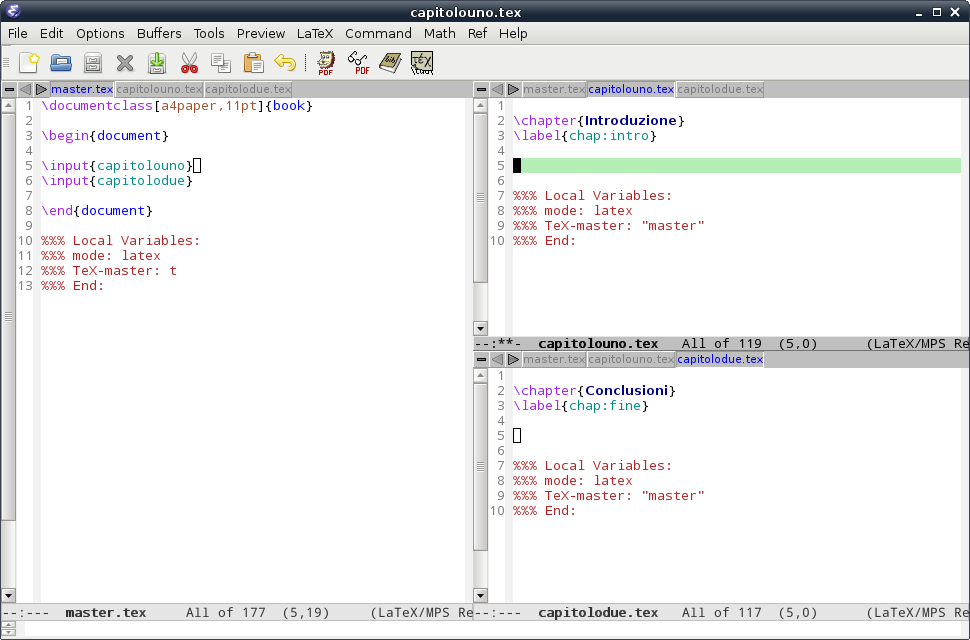
\includegraphics[width=\textwidth]{complesso}
  \caption{Lo schema di un documento complesso suddiviso in più file.  Il
    \emph{frame} è diviso in tre \emph{windows}.}
  \label{fig:complex}
\end{figure}

Per fare in modo che all'apertura di un nuovo documento ci venga chiesto se il
file debba essere o no un file \emph{master}, si deve scrivere
\begin{lstlisting}
(setq-default TeX-master nil)
\end{lstlisting}
nel file \filestyle{.emacs} (si veda il capitolo~\ref{chap:personal}).


\section{Le variabili locali}
\label{sec:variabili:locali}

Abbiamo già accennato alle variabili locali nel paragrafo precedente.  Ora
vediamo la questione un po' più a fondo. Va detto subito che ogni volta che si
aggiunge una variabile locale si deve ricaricare il file perché questa sia
riconosciuta.  Questo può essere fatto aprendo e chiudendo \emacs, oppure, più
semplicemente, eseguendo \verb|M-x revert-buffer RET yes RET|.

Si consiglia di impostare le variabili locali con la modalità di inserimento tra
\verb|%%% Local Variables:| e \verb|%%% End:| alla fine del file.  Alle già
citate \verb|mode: latex| e \verb|TeX-master: t| se ne aggiungono diverse altre
molto utili in un documento \filestyle{.tex}.  Alcune di queste sono messe a
disposizione da \emacs\ e altre da \auctex.

Se per esempio si vuole impostare la codifica del file sorgente a un particolare
valore, \emacs\ mette a disposizione la variabile \verb|coding|, che in questo
documento è impostata come \verb|coding: utf-8| per scrivere con la codifica
Unicode a $8$~bit.  Un altro valore comune è per esempio \verb|coding: latin-1|.
Per vedere tutte le codifiche supportate da \emacs\ basta dare
\verb|M-x list-coding-systems|.

Tra le varie variabili locali di \auctex\ invece, segnaliamo qui quella che
riguarda il motore di tipocomposizione. La variabile è \verb|TeX-engine:|, che
può essere impostata, per esempio, come \verb|TeX-engine: xetex| per far sì che
la sequenza \verb|C-c C-c| lanci direttamente la composizione con \XeLaTeX.

Infine, se si è incerti sul nome della variabile da aggiungere e si ha timore di
sbagliare, si può scrivere \verb|M-x add-file-local-variable|, poi \verb|RET| e
quindi la variabile, aiutandosi magari con l'autocompletamento (tasto
\keys{\tab}\,).


\section{Sinossi delle principali scorciatoie}
\label{sec:sinossi:sco}

\emacs\ offre un'infinità di combinazioni di tasti per eseguire operazioni
banali e meno banali, tanto che scriverle tutte sarebbe impossibile.  Va da sé,
dunque, che per usare il programma non serve ricordarle tutte, ma solo le
principali, mostrate nella tabella~\ref{tab:cheat-sheet}, che con l'uso
quotidiano saranno automaticamente memorizzate.  Per approfondire il discorso si
possono consultare anche le \emph{Reference Card}, disponibili in genere nella
propria cartella di installazione.

\begin{longtable}{>{\ttfamily}l>{\ttfamily}lp{0.35\textwidth}}
  % intestazione iniziale
  \caption{\emph{Scorciatoia} è la combinazione di tasti da premere per ottenere
    il risultato descritto nell'ultima colonna.  La seconda colonna riporta la
    \emph{funzione}, da eseguire con \texttt{M-x}, a cui è legata quella
    particolare combinazione di tasti.}
  \label{tab:cheat-sheet} \\
  \toprule
  {\normalfont\scshape Scorciatoia} & {\normalfont\scshape Funzione} &
  \textsc{Effetto} \\
  \midrule
  \endfirsthead
  % intestazione normale
  \multicolumn{3}{l}{\footnotesize\itshape
    Continua dalla pagina precedente} \\
  \toprule
  {\normalfont\scshape Scorciatoia} & {\normalfont\scshape Funzione} &
  \textsc{Effetto} \\
  \midrule
  \endhead
  % piede normale
  \midrule
  \multicolumn{3}{r}{\footnotesize\itshape
    Continua nella prossima pagina} \\
  \endfoot
  % piede finale
  \bottomrule
  \multicolumn{3}{r}{\footnotesize\itshape
    Si conclude dalla pagina precedente} \\
  \endlastfoot
  % corpo della tabella
  C-x C-f & find-file & Apre il file da specificare nel minibuffer \\
  C-x C-s & save-buffer & Salva il buffer attuale \\
  C-x C-w & write-file & Salva il file attuale nel file indicato nel minibuffer
  \\
  C-x C-c & - & Chiede se salvare i buffer aperti e
  chiude \emacs \\
  C-g & keyboard-quit & Interrompe il comando in esecuzione \\
  C-x u & undo & Annulla l'ultima operazione \\
  \midrule
  \multicolumn{3}{c}{Ricerca e sostituisci} \\
  \midrule
  C-s & isearch-forward & Ricerca incrementale in avanti \\
  C-r & isearch-backward & Ricerca incrementale indietro \\
  M-g g & goto-line & Sposta il cursore alla riga specificata nel minibuffer \\
  M-\% & query-replace & Ricerca e sostituzione \\
  %\midrule
  \multicolumn{3}{c}{Copia e incolla} \\
  \midrule
  M-w & kill-ring-save & Copia la regione selezionata \\
  C-y & yank & Incolla l'ultima selezione \\
  C-w & kill-region & Taglia la regione selezionata \\
  C-k & kill-line & Taglia il resto della riga attuale \\
  \midrule
  \multicolumn{3}{c}{Aiuto} \\
  \midrule
  C-h ? & help-for-help & Apre una finestra di aiuto \\
  C-h k & describe-key & Mostra la documentazione della combinazione di tasti
  che viene successivamente premuta \\
  C-h f & describe-function & Mostra la documentazione della funzione
  specificata nel minibuffer \\
  \midrule
  \multicolumn{3}{c}{Navigazione fra i buffer} \\
  \midrule
  C-x b & switch-to-buffer & Cambia buffer visualizzato \\
  C-x C-b & list-buffers & Mostra l'elenco dei buffer \\
  C-x k & kill-buffer & Chiude il buffer specificato nel minibuffer \\
  \midrule
  \multicolumn{3}{c}{``Window''} \\
  \midrule
  C-x 2 & - & Divide la ``window'' attuale in due, verticalmente \\
  C-x 3 & - & Divide la ``window'' attuale in due, orizzontalmente \\
  C-x o & other-window & Sposta il cursore nella ``window'' successiva \\
  C-x 0 & delete-window & Chiude la ``window'' attuale \\
  C-x 1 & - & Chiude tutte le ``windows'' tranne quella attuale \\
\end{longtable}

\chapter{Personalizzare \emacs{} e \auctex}
\label{chap:personal}

In questo capitolo vedremo alcune personalizzazioni utili quando si lavora con
documenti \LaTeX{}.  Per modificare le impostazioni relative ad \auctex{} si può
dare \verb!M-x customize-group RET AUCTeX RET!.  In questo modo si aprirà un
buffer in cui modificare le opzioni desiderate tramite l'interfaccia.

Di seguito si suggeriscono alcune porzioni di codice Elisp per
personalizzare \emacs{}, da inserire nel file di inizializzazione
\filestyle{.emacs}.  Per rendere effettive le modifiche si ricordi di riavviare
il programma.
% NOTA: in realtà non è strettamente necessario riavviare Emacs, ma nel 99%
% dei casi dovrebbe essere sufficiente valutare il buffer .emacs dando `M-x
% eval-buffer' e poi riavviare AUCTeX nel buffer con `C-u C-c C-n'.

Per fare in modo che \auctex\ conosca i pacchetti \LaTeX\ caricati, e di
conseguenza fornire le funzioni di autocompletamento per le macro, bisogna
permettergli di effettuare il parsing del documento aggiungendo nel proprio file
\filestyle{.emacs} il seguente codice:
\begin{lstlisting}
(setq TeX-parse-self t) ; Attiva parsing al caricamento
(setq TeX-auto-save  t) ; Attiva parsing al salvataggio
\end{lstlisting}
In questo modo verrà creata una cartella \verb!auto! nella cartella di lavoro,
in cui verranno registrate le informazioni sul proprio documento \LaTeX{} (se
invece non si desidera affollare inutilmente le proprie cartelle, non si
attivino le due opzioni appena descritte).

\auctex{} conosce le macro dei pacchetti principali, ma naturalmente non conosce
\emph{tutti} i pacchetti. Però gli si può far analizzare tutti i file di stile
della propria distribuzione \LaTeX{} dando \verb!M-x TeX-auto-generate-global!.
In questo modo verrà automaticamente aggiunto il supporto a tutti i pacchetti
(tranne quelli troppo complicati e quelli basati su \LaTeX{}3).  L'operazione
può richiedere alcuni minuti, soprattutto alla prima esecuzione.  Se un
pacchetto non è stato correttamente analizzato da \auctex, si possono aggiungere
a mano le relative macro al momento di caricare il pacchetto in questione.  Per
esempio, uno dei pacchetti basati su \LaTeX{}3 è \packstyle{siunitx}.  Il
seguente codice aggiunto al file \filestyle{.emacs} informerà \auctex\ che
questo pacchetto definisce i comandi \cs{SI}, \cs{si}, \cs{ang} e \cs{num}, dei
quali il primo accetta due argomenti e gli ultimi tre solo uno:
\begin{lstlisting}
(eval-after-load "tex"
  '(TeX-add-style-hook
    "siunitx"
    (lambda ()
      (TeX-add-symbols
       '("SI" 2)
       '("si" 1)
       '("ang" 1)
       '("num" 1)))))
\end{lstlisting}

Talvolta, in un documento \LaTeX{} non si carica un certo pacchetto \packstyle{B}
poiché è automaticamente caricato da un altro pacchetto \packstyle{A}, effettivamente
presente nel preambolo. In questi casi, però, \auctex{} potrebbe non rendersene
conto e dunque non fornire l'autocompletamento delle macro del pacchetto
\packstyle{B}, anche se correttamente supportato. Supponiamo inoltre che insieme a
\packstyle{B}, il pacchetto \packstyle{A} carichi anche i pacchetti
\packstyle{C} e \packstyle{D}. Per ovviare a questo problema, si può inserire nel
file d'inizializzazione il seguente codice:
\begin{lstlisting}
(eval-after-load "tex"
  '(TeX-add-style-hook
    "A"
    (lambda ()
      (TeX-run-style-hooks "B" "C" "D"))))
\end{lstlisting}
Per esempio, il pacchetto \packstyle{siunitx} carica automaticamente i pacchetti
\packstyle{array} e \packstyle{amstext} e quindi non serve caricarli ulteriormente.
Per farlo sapere ad \auctex,
possiamo completare il codice precedente come segue:
\begin{lstlisting}
(eval-after-load "tex"
  '(TeX-add-style-hook
    "siunitx"
    (lambda ()
      (TeX-add-symbols
       '("SI" 2)
       '("si" 1)
       '("ang" 1)
       '("num" 1)
      (TeX-run-style-hooks "array" "amstext")))))
\end{lstlisting}

Quando si inseriscono gli ambienti \ambstyle{figure} e \ambstyle{table} con la
combinazione di tasti \verb|C-c C-e table|, verrà data la possibilità di
scrivere una didascalia, inserita nel sorgente \LaTeX\ usando il classico
comando \verb|\caption|.  In maniera predefinita \auctex\ aggiunge il
\verb|\caption| dopo la figura o la tabella, però è possibile indicare per quali
ambienti si preferisce inserire la didascalia all'inizio elencandoli nella
variabile \verb|LaTeX-top-caption-list|.  Per esempio, se si vuole inserire la
didascalia prima di una tabella, bisogna aggiungere nel proprio
\filestyle{.emacs} il seguente codice
\begin{lstlisting}
(setq LaTeX-top-caption-list '("table"))
\end{lstlisting}

Se si è soliti suddividere i propri documenti \LaTeX{} in più file da includere
nel file principale con i comandi \verb!\input! o \verb!\include!, può essere
utile aggiungere al file \filestyle{.emacs}
\begin{lstlisting}
(setq-default TeX-master nil)
\end{lstlisting}
In questo modo, all'apertura del documento \emacs{} chiederà qual è il
file principale associato sul quale saranno eseguiti i comandi di
composizione.

Se si usa spesso \LaTeX{} per comporre documenti matematici, potrebbe essere
utile attivare la modalità \verb!LaTeX-math-mode! con \verb!C-c ~! oppure con il
comando \verb!M-x LaTeX-math-mode!.  In questo modo, per esempio, per inserire
il simbolo \verb!\alpha! si potrà usare la scorciatoia \verb!` a!.  L'elenco
delle altre scorciatoie per i simboli può essere consultato dal menù
\verb!Math! nella barra dei menù.  Per attivare automaticamente questa modalità
ogni volta che si apre un documento \LaTeX, bisogna aggiungere
\begin{lstlisting}
(add-hook 'TeX-mode-hook 'LaTeX-math-mode)
\end{lstlisting}
al file \filestyle{.emacs}.

Il codice
\begin{lstlisting}
(setq TeX-electric-sub-and-superscript t)
\end{lstlisting}
aggiunto al file \filestyle{.emacs}, permette di aggiungere automaticamente una
coppia di parentesi graffe \verb!{}! scrivendo i simboli \verb!_! e
\verb!^! in modalità matematica.

Normalmente, la pressione di \verb!RET! in un sorgente \LaTeX{} aggiunge
semplicemente una nuova riga. Se si vuole che la nuova riga sia anche
automaticamente rientrata, bisogna premere \verb!C-j!.  Per ottenere il rientro
con il semplice \verb!RET!, basta aggiungere il seguente codice al file
d'inizializzazione
\begin{lstlisting}
(setq TeX-newline-function 'newline-and-indent)
\end{lstlisting}
Se si utilizza la funzione \verb!reindent-then-newline-and-indent! al posto di
\verb!newline-and-indent! si avrà, in più, il rientro sulla riga corrente.

\emacs\ permette di limitare automaticamente il numero di caratteri per riga di
codice in un documento attivando la modalità \verb|auto-fill-mode| con la
combinazione di tasti \verb|M-x auto-fill-mode RET|.  È possibile riformattare
un paragrafo mediante la funzione \verb|M-x fill-paragraph RET| che è legata
alla scorciatoia \verb|M-q|.  Se si vuole attivare automaticamente la modalità
\verb|auto-fill-mode| ogni volta che si apre un documento \LaTeX\ è sufficiente
aggiungere questo codice al proprio \filestyle{.emacs}:
\begin{lstlisting}
(add-hook 'LaTeX-mode-hook 'turn-on-auto-fill)
\end{lstlisting}
Il numero massimo di caratteri che devono essere contenuti in ciascuna riga è
definito nella variabile \verb|fill-column| il cui valore predefinito è 70.  Se
lo si vuole cambiare, per esempio in 80, bisogna aggiungere il seguente codice
al proprio \filestyle{.emacs}:
\begin{lstlisting}
(setq-default fill-column 80)
\end{lstlisting}
La variabile \verb|fill-column| può essere impostata anche come variabile
locale.

\bibliography{guidaemacsauctex}

\end{document}

%%% Local Variables:
%%% mode: latex
%%% coding: utf-8
%%% TeX-master: t
%%% fill-column: 80
%%% time-stamp-pattern: "13/\\\\ProvidesFile{.*}\\[%:y/%02m/%02d v"
%%% End:

% LocalWords:  mirror OS For dmg Git Fast Version Control System clonare git
% LocalWords:  clone
